\documentclass[aspectratio=169,9pt]{beamer}

\usetheme{metropolis}
\usepackage{fontspec}
\setsansfont{DejaVu Sans}
\usepackage{amsmath,amssymb,bm}
\usepackage{booktabs}
\usepackage{tikz}
\usepackage{tikz-3dplot}
\usetikzlibrary{
  arrows.meta, positioning, shapes.geometric, fit, backgrounds,
  calc, decorations.pathreplacing, decorations.markings, patterns, 3d
}
\usepackage{pgfplots}
\pgfplotsset{compat=1.18}
\usepackage{xcolor}
\usepackage{graphicx}
\usepackage{mathtools}
\usepackage{mdframed}
\usepackage{array}
\usepackage{pifont}
\usepackage{listings}
\usepackage{fontawesome5}
\usepackage[numbers,compress]{natbib}
\renewcommand{\bibfont}{\tiny}
\newcommand{\cmark}{\ding{51}}
\newcommand{\xmark}{\ding{55}}

%% ─── Color Palette: "Music Bright" ─────────────────────────────────
\definecolor{mprimary}{HTML}{6C3FC0}   % Violet sáng hơn
\definecolor{maccent}{HTML}{FF9F1C}    % Amber ấm
\definecolor{mgood}{HTML}{2EC4B6}      % Teal sáng
\definecolor{mbad}{HTML}{E5484D}       % Coral (giữ)
\definecolor{mgray}{HTML}{8E8E9A}      % Neutral gray
\definecolor{mdark}{HTML}{2D2640}      % Aubergine nhạt hơn
\definecolor{mlight}{HTML}{F5F0FF}     % Lavender nhạt — nền frametitle MỚI
\definecolor{mlightgold}{HTML}{FFF4E0}
\definecolor{mlightsage}{HTML}{E6F8F5}
\definecolor{mlightred}{HTML}{FDE8E8}

\setbeamercolor{frametitle}{bg=mlight, fg=mprimary}
\setbeamercolor{progress bar}{fg=mprimary}
\setbeamercolor{structure}{fg=mprimary}
\setbeamercolor{title separator}{fg=maccent}

%% ─── mdframed Box Styles ─────────────────────────────────────────────────────
\newmdenv[
  topline=false, bottomline=false, rightline=false,
  linewidth=3pt, linecolor=mprimary!60,
  innerleftmargin=10pt, innerrightmargin=6pt,
  innertopmargin=5pt, innerbottommargin=5pt,
  backgroundcolor=mlight
]{primarybox}

\newmdenv[
  topline=false, bottomline=false, rightline=false,
  linewidth=3pt, linecolor=mgood!70,
  innerleftmargin=10pt, innerrightmargin=6pt,
  innertopmargin=5pt, innerbottommargin=5pt,
  backgroundcolor=mlightsage
]{goodbox}

\newmdenv[
  topline=false, bottomline=false, rightline=false,
  linewidth=3pt, linecolor=mbad!70,
  innerleftmargin=10pt, innerrightmargin=6pt,
  innertopmargin=5pt, innerbottommargin=5pt,
  backgroundcolor=mlightred
]{badbox}

\newmdenv[
  topline=false, bottomline=false, rightline=false,
  linewidth=3pt, linecolor=maccent!80,
  innerleftmargin=10pt, innerrightmargin=6pt,
  innertopmargin=5pt, innerbottommargin=5pt,
  backgroundcolor=mlightgold
]{accentbox}

%% ─── Takeaway Banner ─────────────────────────────────────────────────────────
\newcommand{\takeaway}[1]{%
  \vfill
  \begin{mdframed}[
    linecolor=maccent, linewidth=1.5pt,
    backgroundcolor=mlightgold,
    innertopmargin=5pt, innerbottommargin=5pt,
    innerleftmargin=10pt, innerrightmargin=10pt,
    roundcorner=3pt, skipabove=4pt, skipbelow=0pt
  ]
  \centering\small\bfseries\color{mprimary} #1
  \end{mdframed}%
}

%% ─── Image placeholder (thay bằng screenshot thật sau) ───────────────
\newcommand{\imgplaceholder}[2][0.9\textwidth]{%
  \begin{tikzpicture}
    \node[draw=mprimary!50, fill=mlight, rounded corners=4pt,
          dashed, line width=1pt, minimum width=#1, minimum height=0.58\textheight,
          align=center, font=\footnotesize\color{mprimary!80}] {%
      \faImage~\textbf{[ẢNH CẦN CHÈN]}\\[4pt]#2};
  \end{tikzpicture}%
}

\newcommand{\eqbars}[1]{%
  \begin{tikzpicture}[baseline]
    \foreach \h in {0.18,0.42,0.28,0.55,0.34,0.48,0.22}{
      \fill[#1] (0,0) rectangle (0.12,\h); \pgftransformxshift{6mm}}
  \end{tikzpicture}}

%% ─── TikZ styles ─────────────────────────────────────────────────────────────
\tikzset{
  pbox/.style={draw=mprimary!50, fill=mlight, rounded corners=3pt,
               minimum height=0.65cm, font=\small, inner sep=5pt},
  gbox/.style={draw=mgood!60, fill=mlightsage, rounded corners=3pt,
               minimum height=0.65cm, font=\small, inner sep=5pt},
  rbox/.style={draw=mbad!60, fill=mlightred, rounded corners=3pt,
               minimum height=0.65cm, font=\small, inner sep=5pt},
  abox/.style={draw=maccent!70, fill=mlightgold, rounded corners=3pt,
               minimum height=0.65cm, font=\small, inner sep=5pt},
  darkbox/.style={draw=mprimary, fill=mprimary!85, text=white, rounded corners=3pt,
                  minimum height=0.7cm, font=\small\bfseries, inner sep=6pt},
  arr/.style={->, thick, mprimary},
  darr/.style={->, dashed, thin, mgray},
  srcbox/.style={draw=maccent!70, fill=mlightgold, rounded corners=3pt,
                 minimum height=0.62cm, font=\scriptsize, inner sep=4pt},
  aibox/.style={draw=maccent, fill=maccent!90, text=white, rounded corners=4pt,
                minimum height=0.7cm, font=\small\bfseries, inner sep=6pt},
}

%% ─── Title ───────────────────────────────────────────────────────────────────
\title{\textbf{World Music Intelligence Monitor}}
\subtitle{Phân tích \& cập nhật bản tin âm nhạc toàn cầu theo thời gian thực}
\author{Nhóm SonicT2All --- Phân tích Dữ liệu Thông minh}
\date{}

\begin{document}

% ─── Slide 0: Title ─────────────────────────────────────────────────────────
\begin{frame}[plain]
\vspace{0.4cm}
\begin{columns}[c]
\column{0.50\textwidth}
  \begin{center}
    {\Huge\bfseries\color{mprimary} World Music\\[4pt] Intelligence Monitor}\\[10pt]
    {\large\itshape\color{mprimary!80} Phân tích \& cập nhật bản tin âm nhạc toàn cầu — realtime}\\[14pt]
    {\large\bfseries SonicT2All}\\[4pt]
    {\small\color{mgray} Phân tích Dữ liệu Thông minh}\\[8pt]
    {\scriptsize\color{mgray} 
      GVHD: TS. Nguyễn Tiến Huy, ThS. Nguyễn Thanh Tình\\[6pt]
      \begin{tabular}{@{}l@{\hspace{6pt}}l@{}}
        Bàng Mỹ Linh          & \texttt{23122009} \\[2pt]
        Lại Nguyễn Hồng Thanh & \texttt{23122018} \\[2pt]
        Phan Huỳnh Châu Thịnh & \texttt{23122019} \\[2pt]
        Nguyễn Gia Bảo        & \texttt{23122015} \\[2pt]
        Nguyễn Ngọc Như Quỳnh & \texttt{23120080} \\
      \end{tabular}
    }\\[10pt]
    \eqbars{maccent}
  \end{center}

\column{0.50\textwidth}
  \begin{center}
    
\includegraphics[width=\linewidth,height=0.72\textheight,keepaspectratio]{slides/figures/music_monitor_cover.png}
  \end{center}
\end{columns}
\end{frame}

% ─── Slide 1: Outline ────────────────────────────────────────────────────────
\begin{frame}{Outline}
\vspace{0.8cm}
\begin{center}
\begin{tikzpicture}[x=2.5cm, y=1cm]
  \tikzstyle{stepbox} = [fill=white, rounded corners=6pt, text width=2.1cm, align=center, inner sep=4pt, minimum height=1.4cm, line width=1pt]
  \tikzstyle{stepnum} = [circle, text=white, font=\footnotesize\bfseries, inner sep=0pt, minimum size=0.6cm]
  
  %% Connecting Line
  \draw[line width=1.5pt, mprimary!20] (0, 1.2) -- (4, 1.2);

  %% Step 1
  \node[stepbox, draw=mprimary] (b1) at (0, -0.2) {\textbf{\color{mprimary}TỔNG QUAN}\\[3pt]\scriptsize Kiến trúc \&\\data pipeline};
  \node[stepnum, fill=mprimary] (n1) at (0, 1.2) {1};
  \draw[thick, mprimary] (n1) -- (b1);

  %% Step 2
  \node[stepbox, draw=mprimary] (b2) at (1, -0.2) {\textbf{\color{mprimary}TRỰC QUAN HÓA}\\[3pt]\scriptsize Dashboard \&\\cảm xúc};
  \node[stepnum, fill=mprimary] (n2) at (1, 1.2) {2};
  \draw[thick, mprimary] (n2) -- (b2);

  %% Step 3
  \node[stepbox, draw=maccent, line width=1.4pt] (b3) at (2, -0.2) {\textbf{\color{maccent}PHÂN TÍCH}\\[3pt]\scriptsize Phân cụm \&\\phát hiện viral \faStar};
  \node[stepnum, fill=maccent] (n3) at (2, 1.2) {3};
  \draw[thick, maccent] (n3) -- (b3);

  %% Step 4
  \node[stepbox, draw=maccent] (b4) at (3, -0.2) {\textbf{\color{maccent}DỰ ĐOÁN}\\[3pt]\scriptsize XGBoost \&\\AI Agent};
  \node[stepnum, fill=maccent] (n4) at (3, 1.2) {4};
  \draw[thick, maccent] (n4) -- (b4);

  %% Step 5
  \node[stepbox, draw=mgood] (b5) at (4, -0.2) {\textbf{\color{mgood}ĐÁNH GIÁ}\\[3pt]\scriptsize Điểm mạnh \&\\hướng phát triển};
  \node[stepnum, fill=mgood] (n5) at (4, 1.2) {5};
  \draw[thick, mgood] (n5) -- (b5);

\end{tikzpicture}
\end{center}

\vspace{0.8cm}
\begin{accentbox}
\centering\small\itshape
Từ dữ liệu thô đa nền tảng $\to$ bản tin âm nhạc thông minh, realtime.
\end{accentbox}
\end{frame}

% ─── SECTION DIVIDER ──────────────────────────────────────────────────────────
\section{TỔNG QUAN \& KIẾN TRÚC}

% ─── Slide 2: Bối Cảnh & Đặt Vấn Đề ───────────────────────────────────────────
\begin{frame}{Bối Cảnh \& Đặt Vấn Đề}

\begin{columns}[c]
\column{0.48\textwidth}
\begin{badbox}
  \textbf{THỰC TRẠNG}\\[4pt]
  \scriptsize
  \faTimes~ \textbf{Phân mảnh:} Dữ liệu rải rác trên YouTube, Last.fm, TikTok, Reddit.\\[4pt]
  \faTimes~ \textbf{Có độ trễ:} Bảng xếp hạng truyền thống phản ứng chậm với trend.\\[4pt]
  \faTimes~ \textbf{Thiếu chiều sâu:} Biết bài hát hot, nhưng không hiểu \textit{tại sao} hot.
\end{badbox}

\vspace{0.3cm}
\begin{goodbox}
  \textbf{GIẢI PHÁP}\\[4pt]
  \scriptsize
  \faCheck~ \textbf{Realtime Pipeline:} Giám sát đa nguồn liên tục.\\[4pt]
  \faCheck~ \textbf{AI/ML Models:} Nhận diện viral \& dự đoán bản hit.\\[4pt]
  \faCheck~ \textbf{LLM Agent:} Đọc hiểu cộng đồng, tóm tắt lý do viral.
\end{goodbox}

\column{0.50\textwidth}
\begin{center}
  \begin{tikzpicture}[every node/.style={font=\scriptsize}, scale=0.85, transform shape]
    \node[aibox, circle, minimum size=1.8cm, align=center, inner sep=0pt] (center) at (0,0) {\faChartLine\\[2pt]Monitor};
    
    \node[srcbox] (s1) at (-2.4, 1.0) {\faYoutube~YouTube};
    \node[srcbox] (s2) at (-1.0, 1.8) {Last.fm};
    \node[srcbox] (s3) at (1.0, 1.8) {\faReddit~Reddit};
    \node[srcbox] (s4) at (2.4, 1.0) {Deezer};
    
    \draw[arr] (s1) -- (center);
    \draw[arr] (s2) -- (center);
    \draw[arr] (s3) -- (center);
    \draw[arr] (s4) -- (center);
    
    \node[pbox, font=\scriptsize, inner sep=4pt] (o1) at (-2.2, -1.4) {Dashboard};
    \node[pbox, font=\scriptsize, inner sep=4pt] (o2) at (0, -2.2) {World Map};
    \node[pbox, font=\scriptsize, inner sep=4pt] (o3) at (2.2, -1.4) {AI Chat};
    
    \draw[darr] (center) -- (o1);
    \draw[darr] (center) -- (o2);
    \draw[darr] (center) -- (o3);
  \end{tikzpicture}
\end{center}
\end{columns}

\vspace{0.4cm}
\takeaway{World Music Monitor: Lời giải cho bài toán phân tích âm nhạc kỷ nguyên số.}

\end{frame}

% ─── Slide 2: Bài Toán & Giải Pháp ───────────────────────────────────────────
\begin{frame}{Tổng Quan Nền Tảng}

\begin{columns}[T]
\column{0.5\textwidth}
\vspace{0.4cm}
\begin{itemize}\footnotesize\setlength\itemsep{10pt}
  \item \textbf{Global Music Intelligence:} Phân tích dữ liệu âm nhạc theo thời gian thực.
  \item \textbf{Hệ sinh thái đa tính năng:} Từ Giám sát tổng quan (Dashboard), Phân cụm thị hiếu (World Map), đến Dự đoán (Prediction).
  \item \textbf{Đa nguồn dữ liệu:} Tích hợp luồng dữ liệu từ YouTube, Deezer, Last.fm và mạng xã hội Reddit.
  \item \textbf{Tích hợp AI Đích thực:} Tiên phong ứng dụng mô hình ngôn ngữ lớn (Gemini) vào hệ thống phân tích.
\end{itemize}

\column{0.46\textwidth}
\begin{center}
  
\includegraphics[width=\linewidth,height=0.3\textheight,keepaspectratio]{slides/figures/bright-mode.png}
  
  \vspace{0.15cm}
  
\includegraphics[width=\linewidth,height=0.3\textheight,keepaspectratio]{slides/figures/dark-mode.png}
\end{center}
\end{columns}

\takeaway{Nền tảng phân tích âm nhạc đa nguồn, đa tính năng, dẫn dắt bởi AI.}

\end{frame}

% ─── Slide 3: Kiến Trúc Hệ Thống ─────────────────────────────────────────────
\begin{frame}{Kiến Trúc Hệ Thống}

\begin{center}
\resizebox{0.9\textwidth}{!}{
\begin{tikzpicture}[every node/.style={font=\scriptsize}, x=1.9cm, y=1.2cm]

  % Layer 1: FRONTEND
  \node[pbox, minimum width=16.5cm, minimum height=1.3cm, fill=mprimary!10, draw=mprimary!40, align=left] (fe) at (0, 2.2) {};
  \node[font=\bfseries\color{mprimary}, anchor=north west, xshift=4pt, yshift=-4pt] at (fe.north west) {FRONTEND \textmd{\scriptsize(Next.js 14 $\cdot$ App Router $\cdot$ TypeScript)}};
  
  \node[pbox, fill=white, minimum height=0.4cm] (d1) at (-2.5, 1.9) {Dashboard};
  \node[pbox, fill=white, minimum height=0.4cm] (d2) at (0, 1.9) {World Map};
  \node[pbox, fill=white, minimum height=0.4cm] (d3) at (2.5, 1.9) {AI Chat};
  \node[font=\scriptsize\color{mgray}, anchor=north east, xshift=-4pt, yshift=-4pt] at (fe.north east) {Vercel $\cdot$ port 3000};

  % Layer 2: BACKEND
  \node[darkbox, minimum width=16.5cm, minimum height=1.3cm, align=left] (be) at (0, 0.6) {};
  \node[font=\bfseries\color{white}, anchor=north west, xshift=4pt, yshift=-4pt] at (be.north west) {BACKEND \textmd{\scriptsize(FastAPI $\cdot$ Python 3.11 $\cdot$ Uvicorn)}};
  
  \node[pbox, fill=white, text=mprimary, minimum height=0.4cm] (b1) at (-3.2, 0.3) {Routers};
  \node[pbox, fill=white, text=mprimary, minimum height=0.4cm] (b2) at (-1.1, 0.3) {Services};
  \node[pbox, fill=white, text=mprimary, minimum height=0.4cm] (b3) at (1.1, 0.3) {AI/ML};
  \node[pbox, fill=white, text=mprimary, minimum height=0.4cm] (b4) at (3.2, 0.3) {Scheduler};
  \node[font=\scriptsize\color{white}, anchor=north east, xshift=-4pt, yshift=-4pt] at (be.north east) {Render.com $\cdot$ port 8000};

  % Layer 3: AI / EXTERNAL
  \node[draw=mgray!50, dashed, rounded corners=3pt, minimum width=7.2cm, minimum height=1.8cm] (ext_left) at (-2.4, -1.55) {};
  \node[font=\scriptsize\color{mgray}, anchor=south west, xshift=4pt, yshift=2pt] at (ext_left.north west) {External Sources};
  
  \node[srcbox] (s1) at (-3.4, -1.2) {Last.fm};
  \node[srcbox] (s2) at (-1.4, -1.2) {\faYoutube};
  \node[srcbox] (s3) at (-3.4, -1.9) {\faReddit};
  \node[srcbox] (s4) at (-1.4, -1.9) {Deezer};

  \node[draw=mgray!50, dashed, rounded corners=3pt, minimum width=7.5cm, minimum height=1.8cm] (ext_right) at (2.4, -1.55) {};
  \node[font=\scriptsize\color{mgray}, anchor=south east, xshift=-4pt, yshift=2pt] at (ext_right.north east) {AI Models};
  
  \node[aibox] (a1) at (1.1, -1.2) {Gemini};
  \node[aibox] (a2) at (3.3, -1.2) {K-Means / XGBoost};
  \node[aibox] (a3) at (2.4, -1.9) {ReAct Agent};

  % Layer 4: DATA LAYER
  \node[pbox, minimum width=16.5cm, minimum height=1.2cm, fill=mprimary!10, draw=mprimary!40, align=left] (db) at (0, -3.1) {};
  \node[font=\bfseries\color{mprimary}, anchor=north west, xshift=4pt, yshift=-4pt] at (db.north west) {DATA LAYER};
  
  \node[pbox, fill=white, minimum height=0.4cm] (db1) at (-2.8, -3.3) {Firebase Firestore};
  \node[pbox, fill=white, minimum height=0.4cm] (db2) at (0, -3.3) {map\_cache.json};
  \node[pbox, fill=white, minimum height=0.4cm] (db3) at (2.8, -3.3) {In-memory cache};

  % Arrows
  \draw[<->, thick, mprimary] (fe.south) -- (be.north) node[midway, right, font=\scriptsize] {HTTP REST + SSE};
  
  \draw[<->, thick, mprimary] (be.south -| ext_left.north) -- (ext_left.north) node[midway, left, font=\scriptsize, fill=white, inner sep=2pt] {HTTP calls};
  \draw[<->, thick, mprimary] (be.south -| ext_right.north) -- (ext_right.north) node[midway, right, font=\scriptsize, fill=white, inner sep=2pt] {HTTP calls};
  
  \draw[<->, thick, mprimary] (be.south) -- (db.north) node[midway, right, font=\scriptsize, fill=white, inner sep=2pt] {Cache IO};

\end{tikzpicture}
}
\end{center}

\vspace{-0.2cm}
\begin{center}
  \tiny\itshape\color{mgray} Kiến trúc 3-tier + lớp AI — mỗi tầng deploy độc lập.
\end{center}

\takeaway{3 tầng tách biệt + lớp AI — dữ liệu chảy một chiều, dễ mở rộng.}

\end{frame}

% ─── Slide 4: Data Pipeline ──────────────────────────────────────────────────
\begin{frame}{Data Pipeline: Đa Nguồn \& Realtime}

\begin{center}
\begin{tikzpicture}[every node/.style={font=\small}, x=2.5cm, y=0.6cm]
  % Sources
  \node[srcbox, minimum width=2cm] (s1) at (0, 1.5) {Last.fm};
  \node[srcbox, minimum width=2cm] (s2) at (0, 0.5) {\faYoutube~YouTube};
  \node[srcbox, minimum width=2cm] (s3) at (0, -0.5) {\faReddit~Reddit};
  \node[srcbox, minimum width=2cm] (s4) at (0, -1.5) {Deezer};
  
  \node[font=\tiny\color{mgray}, below=2pt of s4] {miễn phí, không cần key};

  % Scheduler
  \node[darkbox, align=center] (sched) at (1.8, 0) {Scheduler\\(APScheduler)};

  % Cache
  \node[draw=mgray!50, dashed, rounded corners=3pt, minimum width=3.2cm, minimum height=2.2cm] (cache_bg) at (3.5, -0.15) {};
  \node[font=\scriptsize\color{mgray}, anchor=south, yshift=2pt] at (cache_bg.north) {Cache Layer};

  \node[pbox, minimum width=2.5cm] (fs) at (3.5, 0.4) {Firebase Firestore};
  \node[pbox, minimum width=2.5cm] (mc) at (3.5, -0.7) {map\_cache.json};

  % Arrows
  \draw[arr] (s1.east) to[out=0, in=180] node[pos=0.45, above, sloped, font=\scriptsize, fill=white, inner sep=1pt] {poll 6h} (sched.west);
  
  \draw [decorate, decoration={brace, amplitude=4pt}, thick, mgray] 
    ([xshift=4pt, yshift=2pt]s2.north east) -- ([xshift=4pt, yshift=-2pt]s4.south east) 
    node [midway, right=4pt, font=\scriptsize\color{mgray}] (brace_node) {on-demand};

  \draw[arr] (brace_node.east) to[out=0, in=180] (sched.west);

  \draw[arr] (sched.east) -- (cache_bg.west);
  
  \node[pbox] (router) at (1.8, 2.4) {Router $\to$ JSON};
  \draw[arr, rounded corners] (cache_bg.north) |- (router.east);
  
\end{tikzpicture}
\end{center}

\vspace{0.1cm}
\begin{itemize}\footnotesize\setlength\itemsep{3pt}
  \item Polling 6h cho Last.fm — tối ưu quota Firebase free tier.
  \item 4 nguồn còn lại fetch on-demand, song song bằng \texttt{asyncio.gather}.
  \item Cache 3 lớp: Firestore (cloud) $\cdot$ file JSON $\cdot$ in-memory.
\end{itemize}

\vspace{0.1cm}
\begin{primarybox}
  \textbf{Vì sao polling, không webhook?}\\[2pt]
  \footnotesize
  Các nền tảng nhạc không cung cấp webhook — polling + cache là lựa chọn thực tế.
\end{primarybox}

\takeaway{5+ nguồn, polling 6h + on-demand, cache 3 lớp — luôn có dữ liệu để hiển thị.}

\end{frame}

% ─── Slide 5: Bảo Mật & Định Danh ────────────────────────────────────────────
\begin{frame}{Bảo Mật \& Định Danh}

\begin{columns}[T]
\column{0.5\textwidth}
\begin{center}
\begin{tikzpicture}[every node/.style={font=\footnotesize}, y=-1.0cm, scale=0.7, transform shape]
  \node[pbox] (user) at (0, 0) {Người dùng};
  
  \node[darkbox] (clerk) at (0, 1.1) {Clerk Middleware};
  
  \node[draw=mgray, dashed, rounded corners=3pt, minimum width=3.2cm, minimum height=0.6cm] (pub) at (-1.8, 2.3) {Route public};
  \node[draw=mgray, dashed, rounded corners=3pt, minimum width=3.2cm, minimum height=0.6cm] (prot) at (2.0, 2.3) {Route protected};
  
  \node[font=\tiny\color{mgray}, below=2pt of pub] {/, /sign-in};
  
  \node[gbox] (pass) at (-1.8, 3.4) {Cho qua};
  \node[darkbox] (auth) at (2.0, 3.4) {auth().protect()};
  
  \node[gbox] (dash) at (2.0, 4.5) {Vào Dashboard};
  
  \node[font=\scriptsize\color{mgray}, align=center] (login) at (4.2, 3.4) {Sign-in\\(chưa login)};
  
  \draw[arr] (user) -- (clerk);
  \draw[arr] (clerk) -- (pub.north);
  \draw[arr] (clerk) -- (prot.north);
  \draw[arr] (pub) -- (pass);
  \draw[arr] (prot) -- (auth);
  \draw[arr] (auth) -- (dash);
  
  \draw[darr] (auth) -- (login);
\end{tikzpicture}
\end{center}

\column{0.48\textwidth}
\vspace{0.3cm}

\begin{primarybox}
  \textbf{Clerk — Identity Platform}\\[4pt]
  \footnotesize
  \faCheck~ SSO: đăng nhập qua Google / Email-Password.\\[4pt]
  \faCheck~ Quản lý session, connected accounts minh bạch.
\end{primarybox}

\vspace{0.4cm}
\begin{goodbox}
  \textbf{Bảo vệ được gì}\\[4pt]
  \footnotesize
  \faLock~ Chặn truy cập trái phép vào Data Pipeline \& AI Chat.\\[4pt]
  \faLock~ Nền móng sẵn sàng cho RBAC (Admin / Viewer).
\end{goodbox}

\end{columns}

\takeaway{Clerk lo định danh \& phân quyền — nhóm tập trung vào phần phân tích.}

\end{frame}

% ─── Slide 6: Hồ Sơ Cá Nhân ──────────────────────────────────────────────────
\begin{frame}{Hồ Sơ Cá Nhân}

\vspace{0.1cm}
\begin{itemize}\footnotesize\setlength\itemsep{4pt}
  \item \textbf{Quản trị hồ sơ toàn diện:} Tích hợp Portal quản lý tài khoản trực quan cho End-user.
  \item \textbf{Định danh liên kết (Connected Accounts):} Kiểm soát và đồng bộ hóa luồng đăng nhập SSO (Google, Github) một cách minh bạch, an toàn.
  \item \textbf{Mở rộng phân quyền (Future-proof RBAC):} Nền móng CSDL người dùng sẵn sàng triển khai phân quyền theo vai trò (Admin / Viewer).
\end{itemize}

\vspace{0.1cm}
\begin{columns}[c]
\column{0.35\textwidth}
  \begin{center}
    
\includegraphics[width=\linewidth,height=0.58\textheight,keepaspectratio]{slides/figures/sign-in.png}
  \end{center}
\column{0.62\textwidth}
  \begin{center}
    
\includegraphics[width=\linewidth,height=0.58\textheight,keepaspectratio]{slides/figures/personal-info.png}
  \end{center}
\end{columns}

\end{frame}

% ─── SECTION DIVIDER ──────────────────────────────────────────────────────────
\section{THU THẬP \& TRỰC QUAN HÓA}

% ─── Slide 6: Dashboard ──────────────────────────────────────────────────────
\begin{frame}{Dashboard: Giám Sát Tổng Quan}

\begin{columns}[T]
\column{0.58\textwidth}
  % [IMG] dashboard-fullpage.png — chụp full trang /dashboard ở light mode
  
\includegraphics[width=\linewidth,height=0.65\textheight,keepaspectratio]{slides/figures/dashboard.png}

\column{0.4\textwidth}
  \vspace{0.2cm}
  \begin{itemize}\footnotesize\setlength\itemsep{8pt}
    \item[\faBell] Live Anomaly Alert — phát hiện spike realtime.
    \item[\faChartBar] Global Top 50 kèm điểm MIS.
  \end{itemize}
  
  \vspace{-0.1cm}
  \begin{accentbox}
    \footnotesize MIS = Plays + Listeners + trọng số xu hướng.
  \end{accentbox}
  \vspace{0.1cm}
  
  \begin{itemize}\footnotesize\setlength\itemsep{8pt}
    \item[\faFilter] Bộ lọc động: Today / This Week / This Month.
    \item[\faThLarge] Unified UI — số liệu thô + AI Briefing trên 1 màn hình.
  \end{itemize}
\end{columns}

\takeaway{Một màn hình — số liệu realtime và bản tin AI cạnh nhau.}

\end{frame}

% ─── Slide 7: Daily Briefing & Phân Tích Cảm Xúc ─────────────────────────────
\begin{frame}{Daily Briefing \& Phân Tích Cảm Xúc}

\begin{columns}[c]
\column{0.28\textwidth}
\begin{center}
\begin{tikzpicture}[every node/.style={font=\footnotesize}, y=-1.3cm, scale=0.9, transform shape]
  \node[srcbox] (s1) at (-1.5, 0) {Last.fm};
  \node[srcbox] (s2) at (0, 0) {Reddit};
  \node[srcbox] (s3) at (1.5, 0) {Deezer};
  
  \node[aibox, align=center] (vader) at (0, 1) {VADER NLP};
  \node[font=\tiny\color{mgray}, below=1pt of vader] {Neg/Neu/Pos};
  
  \node[pbox] (json) at (0, 2.2) {JSON tổng hợp};
  
  \node[aibox, align=center] (gemini) at (0, 3.2) {Gemini 3.1};
  
  \node[gbox, align=center] (out) at (0, 4.2) {Bản tin};
  
  \draw[arr] (s2) -- (vader);
  \draw[arr] (vader) -- (json);
  \draw[arr, rounded corners=4pt] (s1.south) |- (json.west);
  \draw[arr, rounded corners=4pt] (s3.south) |- (json.east);
  \draw[arr] (json) -- (gemini);
  \draw[arr] (gemini) -- (out);
\end{tikzpicture}
\end{center}

\column{0.70\textwidth}
\begin{itemize}\footnotesize\setlength\itemsep{8pt}
  \item \textbf{Đầu vào:} Top Charts + Reddit (VADER Sentiment) $\to$ Đóng gói JSON.
  \item \textbf{Đầu ra:} Bản tin tự động (Tổng quan, Viral Alert, Dự báo tuần tới).
\end{itemize}

\vspace{0.3cm}
\begin{center}
  
\includegraphics[width=\linewidth,height=0.7\textheight,keepaspectratio]{slides/figures/daily-briefing.png}
\end{center}
\end{columns}

\end{frame}

% ─── Slide 9: Trực Quan Hóa & Phân Tích ──────────────────────────────────────
\begin{frame}{Trực Quan Hóa \& Phân Tích}

\begin{center}
  
\includegraphics[width=\linewidth,height=0.62\textheight,keepaspectratio]{slides/figures/market-insight.png}
\end{center}

\vspace{-0.2cm}
\begin{columns}[T]
\column{0.32\textwidth}
\begin{itemize}\scriptsize\setlength\itemsep{2pt}
  \item \textbf{Multi-source:}\\ Last.fm, YT, Deezer.
\end{itemize}
\column{0.32\textwidth}
\begin{itemize}\scriptsize\setlength\itemsep{2pt}
  \item \textbf{Hit Prediction:}\\ Radar, Buzz, Hit Score.
\end{itemize}
\column{0.32\textwidth}
\begin{itemize}\scriptsize\setlength\itemsep{2pt}
  \item \textbf{Realtime:}\\ Cập nhật thời gian thực.
\end{itemize}
\end{columns}

\takeaway{Gom mọi góc nhìn từ số liệu thô đến dự đoán AI lên cùng một màn hình.}

\end{frame}

% ─── Slide 10: Phân Phối Dữ Liệu ─────────────────────────────────────────────
\begin{frame}{Phân Phối Dữ Liệu}

\begin{columns}[c]
\column{0.65\textwidth}
\begin{center}
  
\includegraphics[width=\linewidth,height=0.72\textheight,keepaspectratio]{slides/figures/phan-phoi-dl.png}
\end{center}

\column{0.33\textwidth}
\begin{itemize}\footnotesize\setlength\itemsep{8pt}
  \item \textbf{Pareto Distribution:}\\ Top 1 chiếm áp đảo $\to$ Quy luật 80/20.
  \item \textbf{Cross-platform:}\\ Tương quan YouTube Views \& Reddit Upvotes.
  \item \textbf{Sentiment Bar:}\\ Phát hiện sớm khủng hoảng truyền thông.
\end{itemize}

\vspace{0.4cm}
\begin{accentbox}
  \scriptsize \textbf{Data Insight:}\\
  Dữ liệu âm nhạc có độ lệch (skewness) rất lớn. Việc phát hiện phân phối giúp quyết định phương pháp \textbf{Log-Transform} khi đưa vào AI.
\end{accentbox}

\end{columns}

\vspace{0.2cm}
\takeaway{Trực quan hoá phân phối không chỉ để báo cáo, mà là cơ sở để thiết kế thuật toán xử lý nhiễu (outliers).}

\end{frame}

% ─── SECTION DIVIDER ──────────────────────────────────────────────────────────
\section{PHÂN TÍCH THÔNG MINH}

% ─── Slide 11: World Map — Phân Cụm Thị Hiếu (K-Means) ───────────────────────
\begin{frame}{World Map — Phân Cụm K-Means}

\begin{columns}[c]
\column{0.36\textwidth}
  \begin{center}
  \begin{tikzpicture}[every node/.style={font=\scriptsize}, y=-0.9cm, scale=0.85, transform shape]
    \node[srcbox, align=center] (b1) at (0, 0) {Deezer chart + Last.fm tags\\(89 quốc gia)};
    \node[pbox] (b2) at (0, 1.2) {Vector 16 thể loại / quốc gia};
    \node[aibox] (b3) at (0, 2.2) {K-Means (k=6)};
    \node[pbox] (b4) at (0, 3.2) {PCA $\to$ toạ độ 2D};
    \node[gbox] (b5) at (0, 4.2) {Nhãn cụm: POP-dominant…};
    
    \draw[arr] (b1) -- (b2);
    \draw[arr] (b2) -- (b3);
    \draw[arr] (b3) -- (b4);
    \draw[arr] (b4) -- (b5);
  \end{tikzpicture}
  
  \vspace{0.2cm}
  \tiny\color{mgray} \itshape Cache map\_cache.json chạy tức thì.
  \end{center}
  
  \vspace{0.1cm}
  \begin{accentbox}
    \scriptsize \textbf{Dị biệt:} VN thuộc cụm Latin-dominant.
  \end{accentbox}

\column{0.62\textwidth}
  \begin{center}
    
\includegraphics[width=\linewidth,height=0.7\textheight,keepaspectratio]{slides/figures/global-map.png}
  \end{center}
  \vspace{0.1cm}
  \begin{center}
    \tiny\color{mgray} \itshape Click quốc gia $\to$ AI Cultural Insight giải thích văn hóa.
  \end{center}
\end{columns}

\end{frame}

% ─── Slide 12: Trending — Phát Hiện Viral ────────────────────────────────────
\begin{frame}{Trending — Phát Hiện Viral}

\begin{columns}[T]
\column{0.45\textwidth}
  \begin{center}
  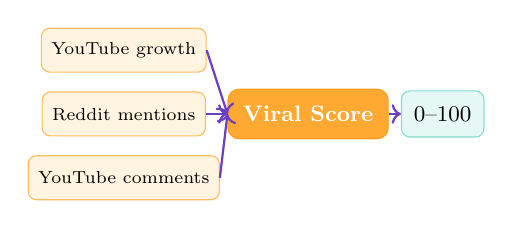
\begin{tikzpicture}[every node/.style={font=\scriptsize}, scale=0.9, transform shape]
    \node[srcbox] (s1) at (0, 0.9) {YouTube growth};
    \node[srcbox] (s2) at (0, 0) {Reddit mentions};
    \node[srcbox] (s3) at (0, -0.9) {YouTube comments};
    
    \node[aibox] (viral) at (2.6, 0) {Viral Score};
    \node[gbox] (out) at (4.5, 0) {0--100};
    
    \draw[arr] (s1.east) -- (viral.west);
    \draw[arr] (s2.east) -- (viral.west);
    \draw[arr] (s3.east) -- (viral.west);
    \draw[arr] (viral) -- (out);
  \end{tikzpicture}
  \end{center}
  
  \vspace{0.2cm}
  \begin{primarybox}
    \footnotesize Viral = 50\% $\cdot$ YouTube + 30\% $\cdot$ Reddit + 20\% $\cdot$ Comments
  \end{primarybox}

\column{0.53\textwidth}
  \begin{itemize}\footnotesize\setlength\itemsep{4pt}
    \item Z-score chuỗi tăng view — phát hiện spike.
    \item Isolation Forest — đánh dấu bài bất thường.
    \item Xếp hạng theo Velocity (vận tốc tăng).
  \end{itemize}
  
  \vspace{0.1cm}
  \begin{center}
    
\includegraphics[width=\linewidth,height=3.5cm,keepaspectratio]{slides/figures/visualize-trending.png}
  \end{center}
  
  \vspace{0.1cm}
  \begin{accentbox}
    \footnotesize \faQuestionCircle~ "Tại sao viral?" — Gemini tổng hợp sự kiện.
  \end{accentbox}
\end{columns}

\end{frame}

% ─── Slide 13: Social Listening ──────────────────────────────────────────────
\begin{frame}{Social Listening}

\vspace{0.1cm}
\begin{itemize}\footnotesize\setlength\itemsep{4pt}
  \item \textbf{Multi-subreddit \& VADER NLP:} Theo dõi r/Music, r/kpop... Phân loại Pos / Neu / Neg \& Mentions 24h.
  \item \textbf{Gemini AI Insight:} Phân tích chủ đề chính, mức độ quan tâm, góc nhìn cộng đồng.
\end{itemize}

\vspace{0.1cm}
\begin{center}
  
\includegraphics[width=0.9\linewidth,height=0.6\textheight,keepaspectratio]{slides/figures/social-listening.png}
\end{center}

\end{frame}

% ─── SECTION DIVIDER ──────────────────────────────────────────────────────────
\section{DỰ ĐOÁN \& AI AGENT}

% ─── Slide 14: Dự Đoán Hit ───────────────────────────────────────────────────
\begin{frame}{Dự Đoán Hit}

\begin{columns}[c]
\column{0.45\textwidth}
\begin{center}
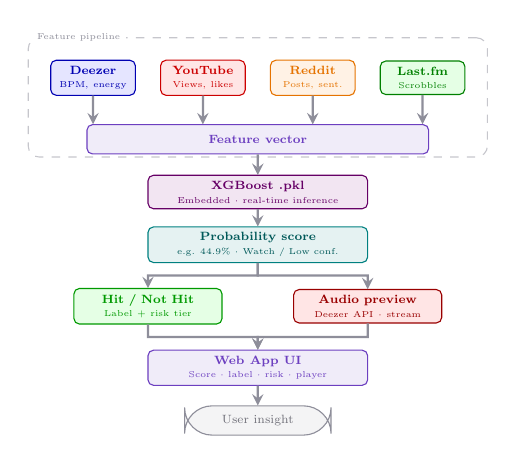
\begin{tikzpicture}[
    every node/.style={font=\scriptsize, rounded corners=2pt},
    arr/.style={->, >=stealth, thick, mgray},
    box/.style={align=center, minimum height=0.6cm},
    scale=0.62, transform shape, y=-0.9cm, x=1.5cm
  ]
  
  \node[box, draw=blue!70!black, fill=blue!10, text=blue!70!black, text width=1.5cm] (deezer) at (-2.25, 0) {\textbf{Deezer}\\ \tiny BPM, energy};
  \node[box, draw=red!80!black, fill=red!10, text=red!80!black, text width=1.5cm] (yt) at (-0.75, 0) {\textbf{YouTube}\\ \tiny Views, likes};
  \node[box, draw=orange!90!black, fill=orange!10, text=orange!90!black, text width=1.5cm] (reddit) at (0.75, 0) {\textbf{Reddit}\\ \tiny Posts, sent.};
  \node[box, draw=green!50!black, fill=green!10, text=green!50!black, text width=1.5cm] (lastfm) at (2.25, 0) {\textbf{Last.fm}\\ \tiny Scrobbles};

  \node[draw=mgray!50, dashed, rounded corners=4pt, inner sep=8pt, fit={(deezer.north west) (lastfm.south east) (0, 1.3)}] (pipeline) {};
  \node[fill=white, text=mgray, font=\tiny, right=2pt] at (pipeline.north west) {Feature pipeline};

  \node[box, draw=mprimary, fill=mprimary!10, text=mprimary, minimum width=7cm, inner sep=4pt] (fvec) at (0, 1.4) {\textbf{Feature vector}};

  \node[box, draw=violet!80!black, fill=violet!10, text=violet!80!black, minimum width=4.5cm] (xgb) at (0, 2.6) {\textbf{XGBoost .pkl}\\ \tiny Embedded $\cdot$ real-time inference};

  \node[box, draw=teal, fill=teal!10, text=teal!70!black, minimum width=4.5cm] (prob) at (0, 3.8) {\textbf{Probability score}\\ \tiny e.g. 44.9\% $\cdot$ Watch / Low conf.};

  \node[box, draw=green!60!black, fill=green!10, text=green!60!black, text width=2.8cm] (hit) at (-1.5, 5.2) {\textbf{Hit / Not Hit}\\ \tiny Label + risk tier};
  \node[box, draw=red!60!black, fill=red!10, text=red!60!black, text width=2.8cm] (audio) at (1.5, 5.2) {\textbf{Audio preview}\\ \tiny Deezer API $\cdot$ stream};

  \node[box, draw=mprimary, fill=mprimary!10, text=mprimary, minimum width=4.5cm] (ui) at (0, 6.6) {\textbf{Web App UI}\\ \tiny Score $\cdot$ label $\cdot$ risk $\cdot$ player};

  \node[box, draw=mgray, fill=mgray!10, text=mgray!80!black, minimum width=3cm, rounded corners=10pt] (user) at (0, 7.8) {User insight};

  \draw[arr] (deezer) -- (deezer |- fvec.north);
  \draw[arr] (yt) -- (yt |- fvec.north);
  \draw[arr] (reddit) -- (reddit |- fvec.north);
  \draw[arr] (lastfm) -- (lastfm |- fvec.north);

  \draw[arr] (fvec) -- (xgb);
  \draw[arr] (xgb) -- (prob);

  \draw[arr] (prob) -- (0, 4.5) -| (hit);
  \draw[arr] (prob) -- (0, 4.5) -| (audio);

  \draw[arr] (hit) |- (0, 5.9) -- (ui);
  \draw[arr] (audio) |- (0, 5.9) -- (ui);

  \draw[arr] (ui) -- (user);

\end{tikzpicture}
\end{center}

\column{0.52\textwidth}
\begin{center}
  
\includegraphics[width=\linewidth,height=4cm,keepaspectratio]{slides/figures/hit-prediction.png}
\end{center}

\vspace{0.2cm}
\begin{minipage}[T]{0.48\linewidth}
\begin{itemize}\scriptsize\setlength\itemsep{4pt}
  \item \textbf{Realtime:}\\ Web App dự đoán.
  \item \textbf{Auto:}\\ Crawl từ 4 nguồn.
\end{itemize}
\end{minipage}%
\hfill
\begin{minipage}[T]{0.48\linewidth}
\begin{itemize}\scriptsize\setlength\itemsep{4pt}
  \item \textbf{Risk \& Score:}\\ \% Hit \& rủi ro.
  \item \textbf{Preview:}\\ Nghe nhạc 30s.
\end{itemize}
\end{minipage}
\end{columns}

\vspace{0.2cm}
\takeaway{Nhập 1 URL $\to$ tự động trích xuất đặc trưng $\to$ XGBoost dự đoán Hit/Flop theo thời gian thực.}

\end{frame}

% ─── Slide 15: Giải Thích Dự Đoán ────────────────────────────────────────────
\begin{frame}{Giải Thích Dự Đoán}

\begin{columns}[c]
\column{0.48\textwidth}
\begin{center}
\begin{tikzpicture}[
    every node/.style={font=\scriptsize, rounded corners=2pt},
    arr/.style={->, >=stealth, thick, mgray},
    box/.style={align=center, minimum height=0.5cm},
    scale=0.48, transform shape, y=-0.85cm, x=1.5cm
  ]

  \node[box, draw=mgray, fill=mgray!10, text=mgray!80!black, minimum width=4cm, rounded corners=10pt] (xgb) at (0, 0) {\textbf{XGBoost output $\cdot$ 44.9\%}};

  \node[box, draw=blue!70!black, fill=blue!10, text=blue!70!black, text width=1.8cm] (shap) at (-2, 1.8) {\textbf{SHAP weights}\\ \tiny Feature import.};
  \node[box, draw=blue!70!black, fill=blue!10, text=blue!70!black, text width=1.8cm] (rank) at (0, 1.8) {\textbf{Feature rank}\\ \tiny Top drivers};
  \node[box, draw=blue!70!black, fill=blue!10, text=blue!70!black, text width=1.8cm] (split) at (2, 1.8) {\textbf{Score split}\\ \tiny +/- contributions};
  
  \node[draw=mgray!50, dashed, rounded corners=4pt, inner sep=6pt, fit={(shap.north west) (split.south east)}] (box1) {};
  \node[text=mgray, font=\tiny, anchor=south west] at (box1.north west) {Giải mã hộp đen};

  \begin{scope}[shift={(0, 4.5)}, x=1cm, y=1cm]
    \foreach \a in {18,90,162,234,306} {
      \draw[mgray!50] (0,0) -- (\a:1.2);
    }
    \draw[fill=blue!20, opacity=0.8, draw=blue, thick]
      (90:1.0) -- (18:0.7) -- (306:1.1) -- (234:0.6) -- (162:0.8) -- cycle;
    \fill[blue] (90:1.0) circle (2pt);
    \fill[blue] (18:0.7) circle (2pt);
    \fill[blue] (306:1.1) circle (2pt);
    \fill[blue] (234:0.6) circle (2pt);
    \fill[blue] (162:0.8) circle (2pt);
    \node[font=\tiny, above] (r1) at (90:1.2) {Memeability};
    \node[font=\tiny, right] (r2) at (18:1.2) {Emotional hook};
    \node[font=\tiny, anchor=north west] (r3) at (306:1.2) {Danceability};
    \node[font=\tiny, anchor=north east] (r4) at (234:1.2) {Lyrics};
    \node[font=\tiny, left] (r5) at (162:1.2) {Shock value};
  \end{scope}
  \node[draw=mgray!50, dashed, rounded corners=4pt, inner xsep=10pt, inner ysep=8pt, fit={(r1) (r2) (r3) (r4) (r5)}] (box2) {};
  \node[text=mgray, font=\tiny, anchor=south west] at (box2.north west) {Radar đa chiều};
  \node[minimum width=2cm, minimum height=2cm] (radar) at (0, 4.5) {};

  \node[box, draw=green!50!black, fill=green!10, text=green!50!black, text width=2cm] (gemini) at (-1.5, 7.5) {\textbf{Gemini}\\ \tiny Reads SHAP + radar};
  \node[box, draw=teal, fill=teal!10, text=teal!70!black, text width=3cm] (semantic) at (1.5, 7.5) {\textbf{Semantic narrative}\\ \tiny Why 44.9\%? $\cdot$ plain lang.};
  \draw[arr] (gemini) -- (semantic);
  \node[draw=mgray!50, dashed, rounded corners=4pt, inner sep=6pt, fit={(gemini.north west) (semantic.south east)}] (box3) {};
  \node[text=mgray, font=\tiny, anchor=south west] at (box3.north west) {LLM phiên dịch};

  \node[box, draw=orange!80!black, fill=orange!10, text=orange!80!black, minimum width=5cm] (risk) at (0, 9.2) {\textbf{Risk tier}\\ \tiny Watch $\cdot$ Low confidence $\cdot$ 44.9\%};

  \node[box, draw=red!70!black, fill=red!10, text=red!70!black, text width=1.8cm] (act1) at (-2, 11) {\textbf{TikTok / Shorts}\\ \tiny Push campaign};
  \node[box, draw=red!70!black, fill=red!10, text=red!70!black, text width=1.8cm] (act2) at (0, 11) {\textbf{Remix hook}\\ \tiny Boost Emotion};
  \node[box, draw=red!70!black, fill=red!10, text=red!70!black, text width=1.8cm] (act3) at (2, 11) {\textbf{Playlist pitch}\\ \tiny Target editorial};

  \node[box, draw=mgray, fill=mgray!10, text=mgray!80!black, minimum width=5cm] (repredict) at (0, 12.4) {\textbf{Re-predict loop}\\ \tiny Apply actions $\to$ re-score $\to$ iterate};
  
  \node[box, draw=mgray, fill=mgray!20, text=mgray!90!black, minimum width=4cm, rounded corners=10pt] (decision) at (0, 13.6) {\textbf{Decision $\cdot$ informed release}};

  \node[draw=mgray!50, dashed, rounded corners=4pt, inner sep=6pt, fit={(act1.north west) (act3.south east) (decision.south)}] (box4) {};
  \node[text=mgray, font=\tiny, anchor=south west] at (box4.north west) {Chiến lược hành động};

  \draw[arr] (xgb) -- (rank);
  \draw[arr] (xgb) -- (0,0.8) -| (shap);
  \draw[arr] (xgb) -- (0,0.8) -| (split);

  \draw[arr] (rank) -- (radar);
  
  \draw[arr] (radar) -- (0, 6.7) -| (gemini);

  \draw[arr] (0, 8.2) -- (risk);

  \draw[arr] (risk) -- (act2);
  \draw[arr] (risk) -- (0, 10.1) -| (act1);
  \draw[arr] (risk) -- (0, 10.1) -| (act3);

  \draw[arr] (act1) |- (0, 11.7) -- (repredict);
  \draw[arr] (act2) -- (repredict);
  \draw[arr] (act3) |- (0, 11.7) -- (repredict);

  \draw[arr] (repredict) -- (decision);

\end{tikzpicture}
\end{center}

\column{0.48\textwidth}
\begin{center}
  
\includegraphics[width=\linewidth,height=3.2cm,keepaspectratio]{slides/figures/visualize-hit.png}
\end{center}

\vspace{0.2cm}
\begin{minipage}[T]{0.48\linewidth}
\begin{itemize}\scriptsize\setlength\itemsep{4pt}
  \item \textbf{Chuyển hóa:}\\ Phân tích dễ hiểu.
  \item \textbf{Radar:}\\ Radar 5 trục.
\end{itemize}
\end{minipage}%
\hfill
\begin{minipage}[T]{0.48\linewidth}
\begin{itemize}\scriptsize\setlength\itemsep{4pt}
  \item \textbf{Phiên dịch:}\\ Gemini đọc trọng số.
  \item \textbf{Đề xuất:}\\ Tư vấn chiến lược.
\end{itemize}
\end{minipage}
\end{columns}

\vspace{0.2cm}
\takeaway{AI không chỉ báo số, mà còn giải thích nguyên nhân và gợi ý hành động.}

\end{frame}

% ─── Slide 16: AI Chat ───────────────────────────────────────────────────────
\begin{frame}{AI Chat}

\begin{columns}[c]
\column{0.40\textwidth}
\begin{center}
\begin{tikzpicture}[
    every node/.style={font=\scriptsize, rounded corners=2pt},
    arr/.style={->, >=stealth, thick, mgray},
    box/.style={align=center, minimum height=0.6cm},
    scale=0.42, transform shape, y=-1.1cm, x=1.5cm
  ]

  \node[box, draw=teal, fill=teal!10, text=teal!80!black, minimum width=6cm, rounded corners=12pt] (user) at (0, 0) {\textbf{Người dùng}\\ \tiny "Tại sao APT trending? Verify từ web"};

  \node[box, draw=purple!80!black, fill=purple!10, text=purple!80!black, minimum width=6cm] (t1) at (0, 1.8) {\textbf{Thought 1 — Lên kế hoạch}\\ \tiny "Cần tìm lý do bài APT viral trên web..."};

  \node[box, draw=blue!70!black, fill=blue!10, text=blue!70!black, minimum width=6cm] (a1) at (0, 3) {\textbf{Action 1 — Gọi tool}\\ \tiny \texttt{web\_search("why is APT trending...")}};

  \node[box, draw=red!70!black, fill=red!10, text=red!70!black, minimum width=6cm] (o1) at (0, 4.2) {\textbf{Observation 1 — Lỗi môi trường}\\ \tiny Error: duckduckgo chưa được cài đặt};

  \node[box, draw=orange!90!black, fill=orange!10, text=orange!90!black, minimum width=6cm] (t2) at (0, 5.4) {\textbf{Thought 2 — Tự phục hồi}\\ \tiny "Dùng kiến thức nội bộ thay thế..."};

  \node[box, draw=mgray, fill=white, dashed, text=mgray, text width=1.2cm] (fallback) at (3.8, 5.4) {Graceful\\fallback};
  \draw[mgray, dashed] (fallback) -- (t2);

  \node[box, draw=green!60!black, fill=green!10, text=green!60!black, minimum width=6cm, rounded corners=12pt] (final) at (0, 7.2) {\textbf{Final answer}\\ \tiny Báo cáo 5 lý do APT thành công};

  \node[draw=mgray!50, dashed, rounded corners=6pt, inner sep=10pt, fit={(t1.north west) (t2.south east) (fallback.east)}] (loop) {};
  \node[fill=white, text=mgray, font=\tiny, right=2pt] at (loop.north west) {ReAct loop};

  \draw[arr] (user) -- (t1);
  \draw[arr] (t1) -- (a1);
  \draw[arr] (a1) -- (o1);
  \draw[arr] (o1) -- (t2);
  \draw[arr] (t2) -- (final);

  \begin{scope}[shift={(0, 8.8)}, x=1cm, y=1cm, every node/.style={font=\tiny, anchor=west}]
    \filldraw[fill=purple!10, draw=purple!80!black] (-4.5, -0.1) rectangle (-4.2, 0.2); \node at (-4.1, 0.05) {Thought};
    \filldraw[fill=blue!10, draw=blue!70!black] (-2.5, -0.1) rectangle (-2.2, 0.2); \node at (-2.1, 0.05) {Action};
    \filldraw[fill=red!10, draw=red!70!black] (-0.5, -0.1) rectangle (-0.2, 0.2); \node at (-0.1, 0.05) {Observation (lỗi)};
    \filldraw[fill=orange!10, draw=orange!90!black] (2.0, -0.1) rectangle (2.3, 0.2); \node at (2.4, 0.05) {Fallback};
    \filldraw[fill=green!10, draw=green!60!black] (4.0, -0.1) rectangle (4.3, 0.2); \node at (4.4, 0.05) {Final answer};
  \end{scope}

\end{tikzpicture}
\end{center}

\column{0.58\textwidth}
\begin{center}
  
\includegraphics[width=\linewidth,height=6.2cm,keepaspectratio]{slides/figures/ai-chat.png}
\end{center}

\vspace{0.1cm}
\begin{center}
  {\scriptsize \faRobot~ \textbf{ReAct Agent:} Tự gọi Tool \quad\quad \faWrench~ \textbf{Tự sửa lỗi:} Fallback nội bộ.}
\end{center}
\end{columns}

\vspace{0.2cm}
\takeaway{Agent tự phân tích, gọi tool và tự xử lý ngoại lệ — vượt giới hạn hỏi đáp tĩnh.}

\end{frame}

% ─── SECTION DIVIDER ──────────────────────────────────────────────────────────
\section{ĐÁNH GIÁ \& KẾT LUẬN}

% ─── Slide 17: Điểm Mạnh & Hạn Chế ───────────────────────────────────────────
\begin{frame}{Điểm Mạnh \& Hạn Chế}

\begin{columns}[T]
\column{0.48\textwidth}
\begin{goodbox}
  \textbf{ĐIỂM MẠNH}\\[6pt]
  \footnotesize
  \faCheck~ Tích hợp đa nguồn: 5 API âm nhạc + AI Gemini trong một hệ thống thống nhất.\\[6pt]
  \faCheck~ Phân tích toàn diện: Clustering, Prediction, Sentiment, Trend Detection.\\[6pt]
  \faCheck~ AI Agent tự chủ: ReAct loop tự gọi tool, tự xử lý lỗi, streaming realtime.
\end{goodbox}

\column{0.50\textwidth}
\begin{badbox}
  \textbf{HẠN CHẾ}\\[6pt]
  \footnotesize
  \faTimes~ API quota hạn chế: YouTube 10K units/ngày, Gemini 14 req/phút free tier.\\[6pt]
  \faTimes~ Chưa scale ngang: Scheduler + API chạy cùng process, chỉ 1 worker.\\[6pt]
  \faTimes~ Chưa có streaming thật: Dữ liệu polling định kỳ, không phải event-driven.
\end{badbox}
\end{columns}

\vspace{0.4cm}
\begin{primarybox}
  \centering\footnotesize
  Sản phẩm hoàn chỉnh end-to-end — nâng cấp hạ tầng và quota là hướng cải thiện rõ nhất.
\end{primarybox}

\takeaway{Mạnh về tích hợp AI \& phân tích — hạn chế chủ yếu ở quota API \& khả năng mở rộng.}

\end{frame}

% ─── Slide 18: Hướng Phát Triển ──────────────────────────────────────────────
\begin{frame}{Hướng Phát Triển}

\vspace{0.8cm}
\begin{center}
\begin{tikzpicture}[every node/.style={font=\footnotesize}, x=2.6cm, y=1cm]
  % Base line
  \draw[thick, mgray!30] (0,0) -- (4,0);
  
  % Nodes
  \node[draw=maccent, fill=maccent!10, text=maccent, circle, minimum size=0.8cm, inner sep=0pt, font=\large] (n1) at (0,0) {\faExpand};
  \node[draw=mprimary, fill=mprimary!10, text=mprimary, circle, minimum size=0.8cm, inner sep=0pt, font=\large] (n2) at (1,0) {\faServer};
  \node[draw=mprimary, fill=mprimary!10, text=mprimary, circle, minimum size=0.8cm, inner sep=0pt, font=\large] (n3) at (2,0) {\faBolt};
  \node[draw=mprimary, fill=mprimary!10, text=mprimary, circle, minimum size=0.8cm, inner sep=0pt, font=\large] (n4) at (3,0) {\faUsersCog};
  \node[draw=mprimary, fill=mprimary!10, text=mprimary, circle, minimum size=0.8cm, inner sep=0pt, font=\large] (n5) at (4,0) {\faBroom};
  
  % Text below nodes
  \node[below=8pt of n1, text=maccent, font=\bfseries\scriptsize, align=center] {Nâng\\quota API};
  \node[below=8pt of n2, text=mgray, font=\scriptsize, align=center] {Tách\\worker};
  \node[below=8pt of n3, text=mgray, font=\scriptsize, align=center] {Event-driven\\streaming};
  \node[below=8pt of n4, text=mgray, font=\scriptsize, align=center] {Phân quyền\\RBAC};
  \node[below=8pt of n5, text=mgray, font=\scriptsize, align=center] {Dọn\\code legacy};
\end{tikzpicture}
\end{center}

\vspace{1cm}
\begin{accentbox}
  \centering\footnotesize
  Ưu tiên \#1: Nâng quota API + tách scheduler $\to$ nền tảng scale cho production thật.
\end{accentbox}

\takeaway{Hướng đi rõ ràng: nâng quota + tách worker + chuyển sang event-driven.}

\end{frame}

% ─── Slide 17: Cảm Ơn — QA & Demo ────────────────────────────────────────────
\begin{frame}[plain]

\vspace{1.5cm}
\begin{center}
  {\Huge\bfseries\color{mprimary} CẢM ƠN ĐÃ LẮNG NGHE}\\[12pt]
  
  {\large\bfseries World Music Intelligence Monitor — SonicT2All}\\[6pt]
  
  {\small\color{mgray} GVHD: TS. Nguyễn Tiến Huy, ThS. Nguyễn Thanh Tình}\\[24pt]
  
  \begin{minipage}{0.35\textwidth}
    \begin{accentbox}
      \centering\large\bfseries QA \& DEMO
    \end{accentbox}
  \end{minipage}\\[24pt]
  
  \eqbars{maccent}
\end{center}

\end{frame}

\end{document}
